\documentclass{article}

\usepackage{graphicx}
\usepackage{tikz}
\usepackage{tikzsymbols}
\usetikzlibrary{calc,patterns,shapes.geometric}
\pagestyle{empty}
\usepackage[margin=0pt]{geometry}
\geometry{papersize={14in,12in}}

\def\centerarc[#1](#2)(#3:#4:#5){\draw[#1] ($(#2)+({#5*cos(#3)},{#5*sin(#3)})$) arc (#3:#4:#5);}

\begin{document}
	\begin{figure}
		\centering
		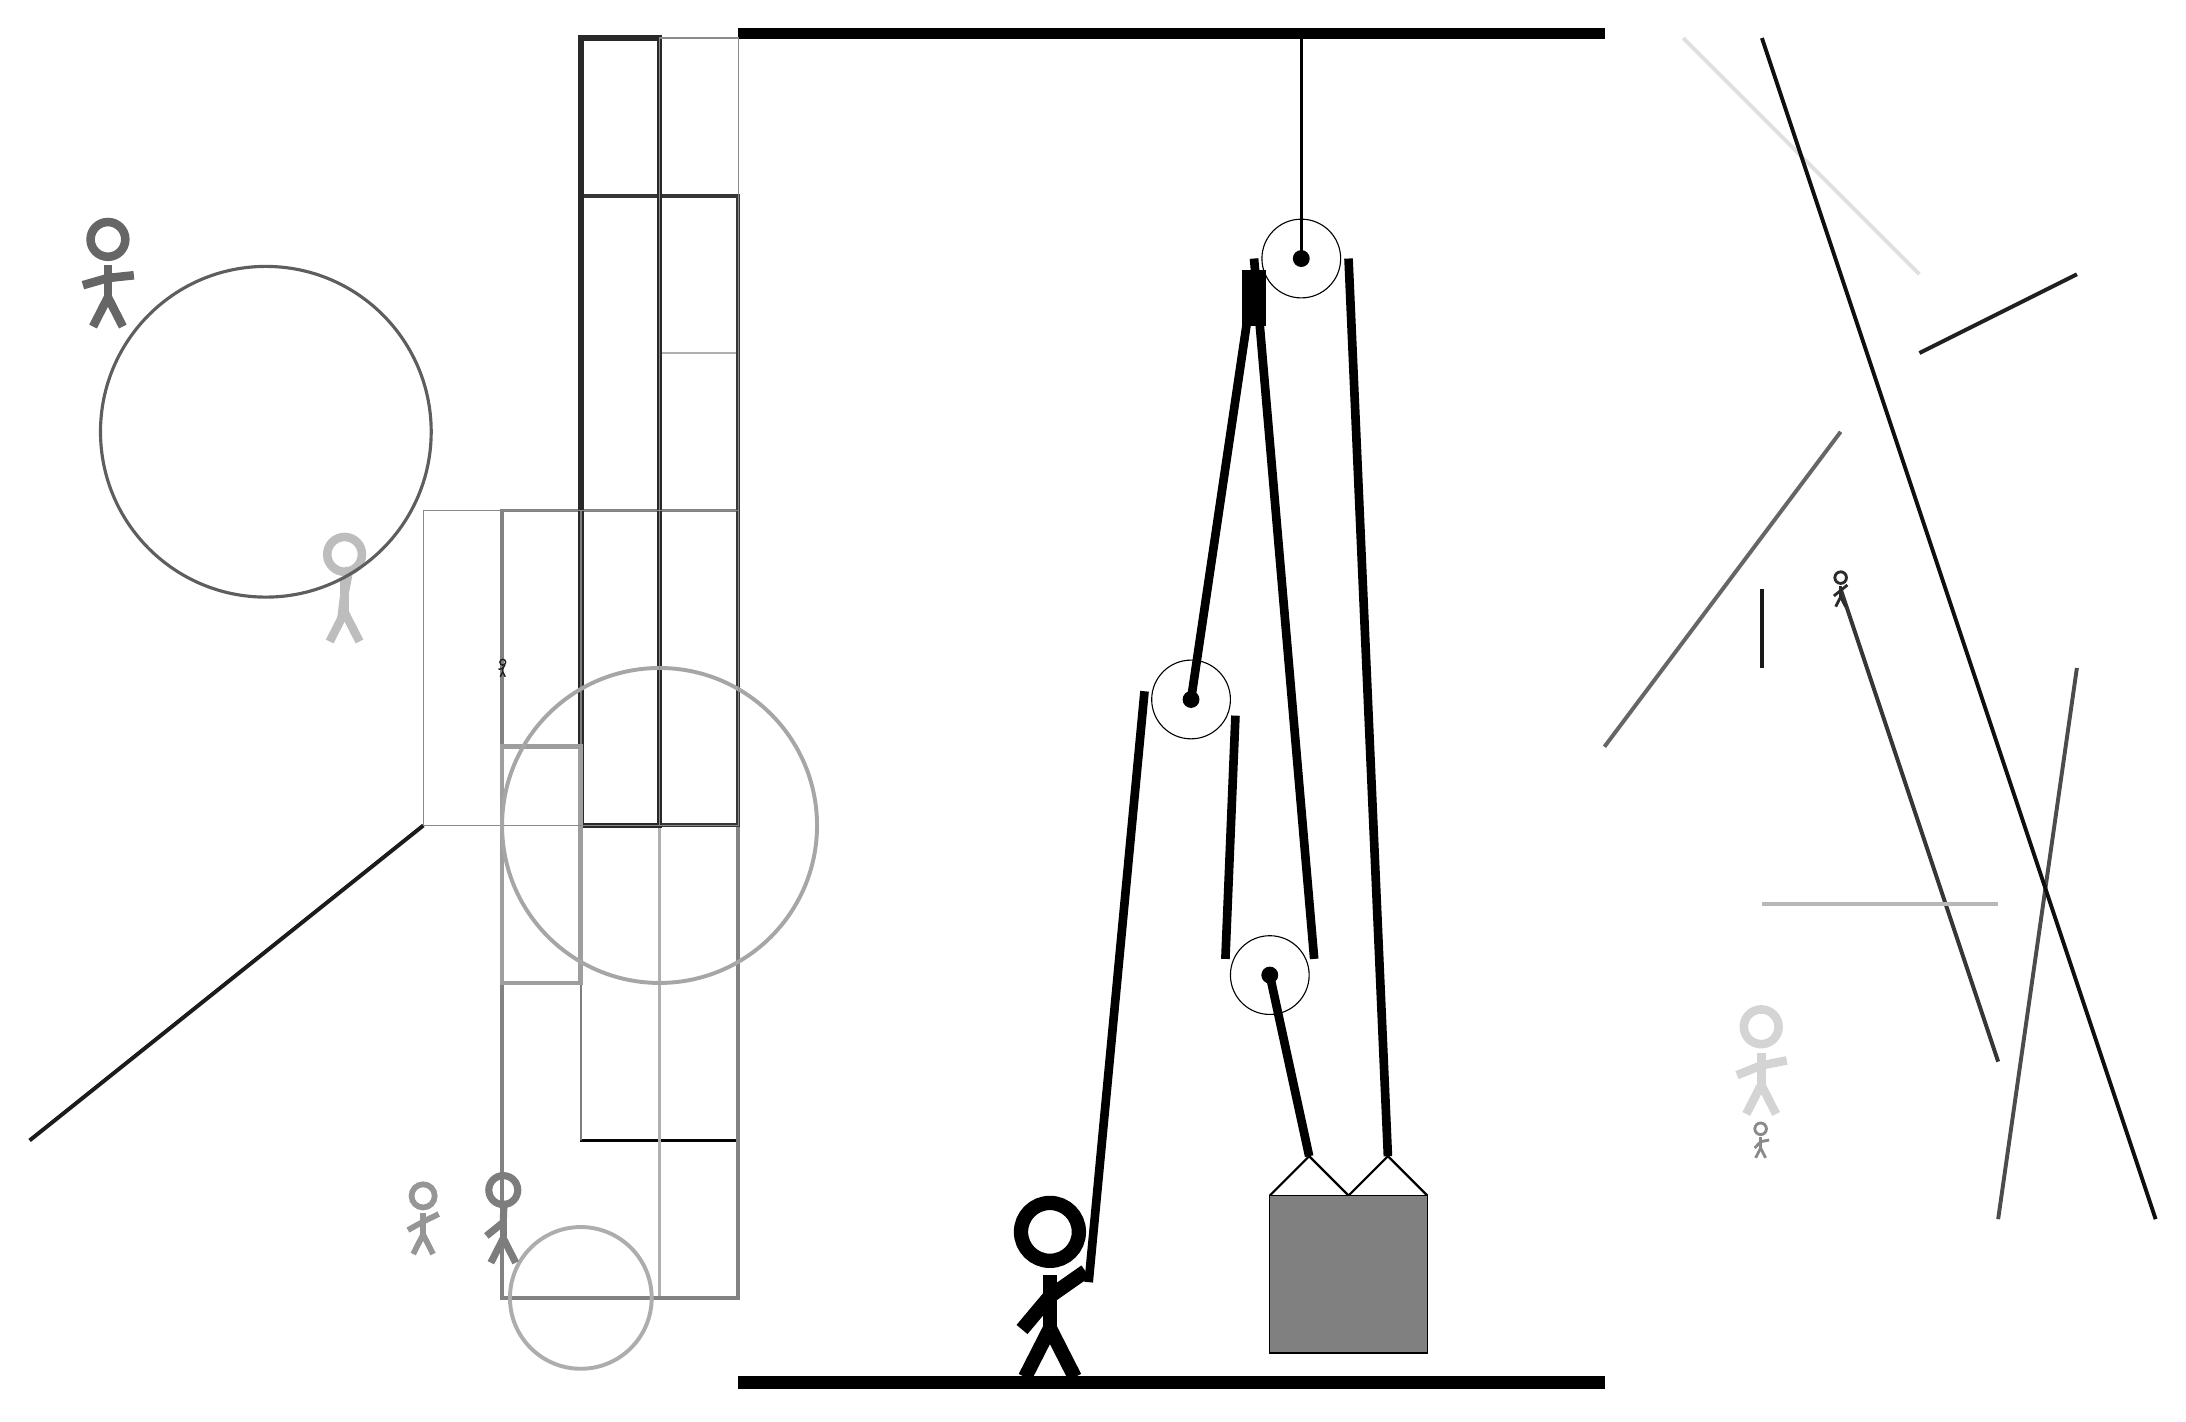
\begin{tikzpicture}
			%%%%% START %%%%%
			
			\draw[fill=black] (-6, 14) rectangle (5, 14.125);
			
			\draw (-0.25, 5.6) circle (0.5);
			\draw[fill=black] (-0.25, 5.6) circle (0.1);
			
			\draw (0.75, 2.1) circle (0.5);
			\draw[fill=black] (0.75, 2.1) circle (0.1);
			
			\draw (1.15, 11.2) circle (0.5);
			\draw[fill=black] (1.15, 11.2) circle (0.1);
			\draw[very thick] (1.15, 11.2) -- (1.15, 14);
			
			\draw[thick]  (0.75, -0.7) -- (1.25, -0.2) -- (1.75, -0.7) -- (2.25, -0.2) -- (2.75, -0.7);
			\draw[fill=black!50] (0.75, -0.7) rectangle (2.75, -2.7);
			
			\draw[line width=1.1mm] (-0.25, 5.6) -- (0.55, 11.0);
			\draw[line width=1.1mm, fill=black](0.45, 10.4) rectangle (0.65, 11.0);
			\draw[line width=1.1mm] (-1.55, -1.8) -- (-0.8409, 5.7042);
			\centerarc[line width=1.1mm](-0.25, 5.6)(-20:170:0.6);
			\draw[line width=1.1mm] (0.3138, 5.3948) -- (0.1862, 2.3052);
			\centerarc[line width=1.1mm](0.75, 2.1)(160:380:0.6);
			\draw[line width=1.1mm] (1.3138, 2.3052) -- (0.55, 11.2);
			\draw[line width=1.1mm](0.75, 2.1) -- (1.25, -0.2);
			\centerarc[line width=1.1mm](1.15, 11.2)(0:180:0.6);
			\draw[line width=1.1mm] (1.75, 11.2) -- (2.25, -0.2);
			
			\node[line width=0.3mm, color=black!17] at (7, 1) {\Strichmaxerl[6][22][11]};
			
			\node[line width=0.7mm, color=black!46] at (7, 0) {\Strichmaxerl[2][47][11]};
			\node[line width=0.3mm, color=black!60] at (-14, 11) {\Strichmaxerl[6][16][6]};
			\draw[line width=0.3mm, color=black!98] (-8, 8) rectangle (-6, 0);
			
			\draw[line width=0.5mm, color=black!12](9, 11) -- (6, 14);
			\draw[line width=0.3mm, color=black!31] (-7, -2) rectangle (-6, 10);
			\draw[line width=0.5mm, color=black!49] (-6, -2) rectangle (-9, 8);
			\node[line width=0.7mm, color=black!87] at (-9, 6) {\Strichmaxerl[1][8][61]};
			\node[line width=0.6mm, color=black!41] at (-10, -1) {\Strichmaxerl[4][29][26]};
			\draw[line width=0.5mm, color=black!79] (-6, 4) rectangle (-8, 12);
			\draw[line width=0.7mm, color=black!84] (-8, 4) rectangle (-7, 14);
			\draw[line width=0.3mm, color=black!51] (-8, 0) rectangle (-8, 8);
			\draw[line width=0.5mm, color=black!60](5, 5) -- (8, 9);
			
			\draw[line width=0.5mm, color=black!89](-10, 4) -- (-15, 0);
			\node[line width=0.2mm, color=black!26] at (-11, 7) {\Strichmaxerl[6][83][79]};
			\draw[line width=0.5mm, color=black!88](9, 10) -- (11, 11);
			
			\draw[line width=0.5mm, color=black!70](10, -1) -- (11, 6);
			\draw [line width=0.5mm, color=black!32](-8, -2) circle (0.9);
			\draw [line width=0.4mm, color=black!63](-12, 9) circle (2.1);
			\draw[line width=0.6mm, color=black!38] (-8, 2) rectangle (-9, 5);
			\draw[line width=0.5mm, color=black!79](8, 7) -- (10, 1);
			\node[line width=0.5mm, color=black!83] at (8, 7) {\Strichmaxerl[2][39][39]};
			\draw[line width=0.5mm, color=black!94](7, 14) -- (12, -1);
			\draw[line width=0.2mm, color=black!46] (-6, 8) rectangle (-10, 4);
			\draw[line width=0.5mm, color=black!28](10, 3) -- (7, 3);
			
			\draw [line width=0.5mm, color=black!35](-7, 4) circle (2.0);
			\node[line width=0.4mm, color=black!51] at (-9, -1) {\Strichmaxerl[5][39][88]};
			\draw[line width=0.6mm, color=black!90] (7, 7) rectangle (7, 6);
			
			\draw[line width=0.2mm, color=black!46] (-7, 14) rectangle (-6, 4);
			
			\node at (-2, -1.9) {\Strichmaxerl[10][50][35]};
			
			\draw[fill=black] (-6, -3) rectangle (5, -3.15);
			
			%%%%% END %%%%%
		\end{tikzpicture}
	\end{figure}	
\end{document}